% !TeX encoding = UTF-8
% !TeX program = lualatex
% !TeX spellcheck = en_US
% !TeX root = thesis.tex

\chapter{Validation studies}
\label{chap:validation_&_verification_study}
\index{validation}
\enlargethispage*{3cm}


\blindtext[1]

\blindtext[1]

%, which is the process of determining that the implementation of a model represents the developer's concept of the model and solution.
Thus, we use validation methods which assess to which quantifiable extent a model is able to represent reality \citep{AIAA1998}. 
%Due to time limitations and preexisting best practice guidelines for environmental flows \citep{Franke2004,Franke2006,Franke2007,Franke2010,Blocken,Ramponi2012} this chapter will focus on validation of the results, such as comparing the results with experimental data in order to quantify accuracy and errors. 
In the validation study, the following elements will be examined \citep{Slater2008,Franke2007}:

\begin{itemize}
%	\item Comparison against experimental datak
	\item Implementation of the model
	\item Consistency
	\item Mesh refinement  
	\item Iterative convergence
	\item Spatial convergence	
	\item Sensitivity of boundary conditions	
\end{itemize}




\enlargethispage*{3cm}
\begin{figure}[!h]
	\centering
	\subfloat[][Residuals very coarse]%
	{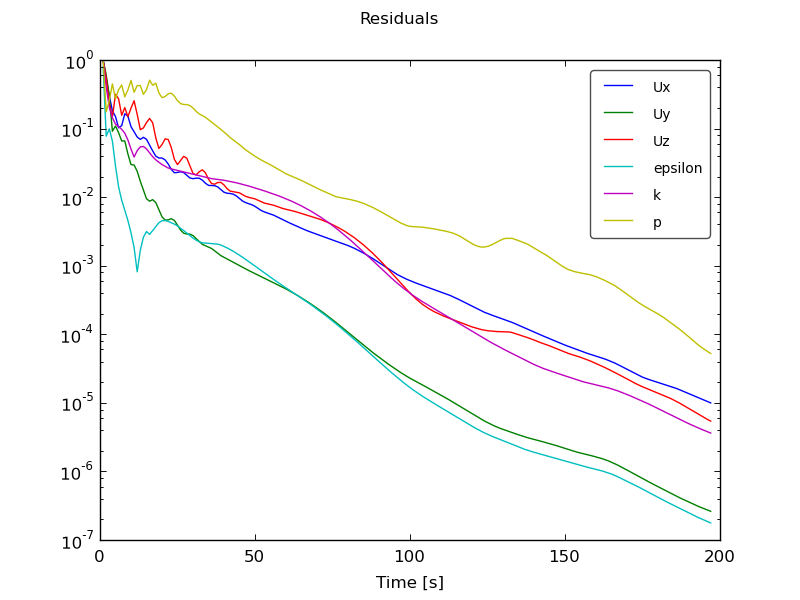
\includegraphics[width=0.48\textwidth, trim= 14mm 2mm 12mm 17mm, clip]{images/plots/validation/iterative_convergence/linear_very_coarse}}\hfil
	\subfloat[][Residuals coarse]%
	{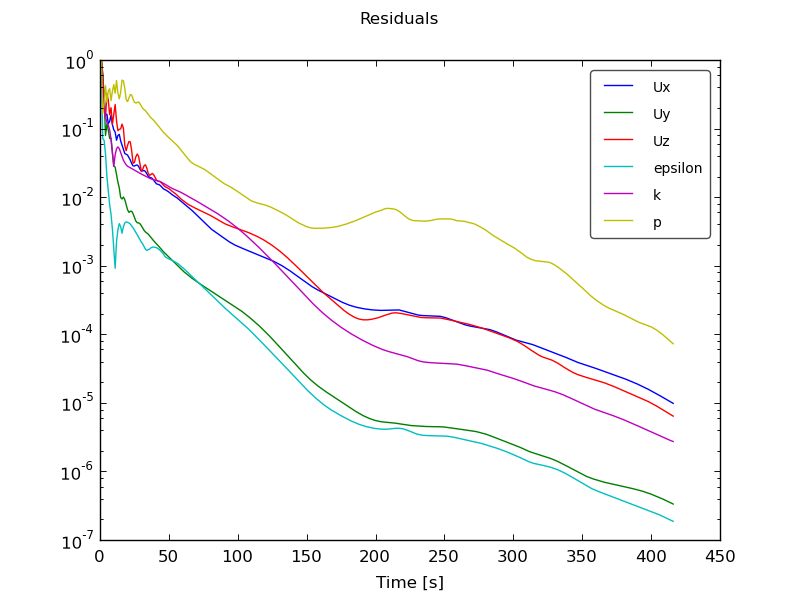
\includegraphics[width=0.48\textwidth, trim= 14mm 2mm 12mm 17mm, clip]{images/plots/validation/iterative_convergence/linear_coarse}}\hfil
	\subfloat[][Residuals normal]%
	{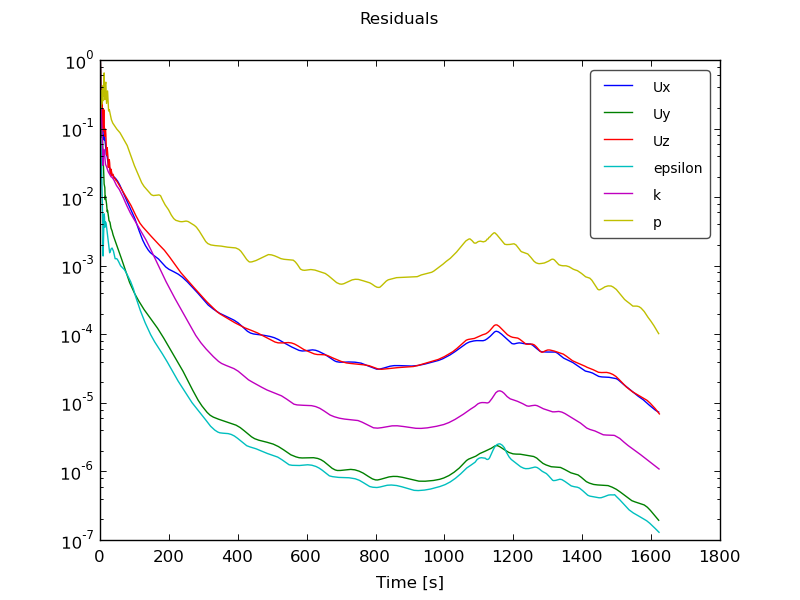
\includegraphics[width=0.48\textwidth, trim= 14mm 2mm 12mm 17mm, clip]{images/plots/validation/iterative_convergence/linear_ref}}\hfil
	\subfloat[][Residuals fine]%
	{\begin{annotatedFigure}
			{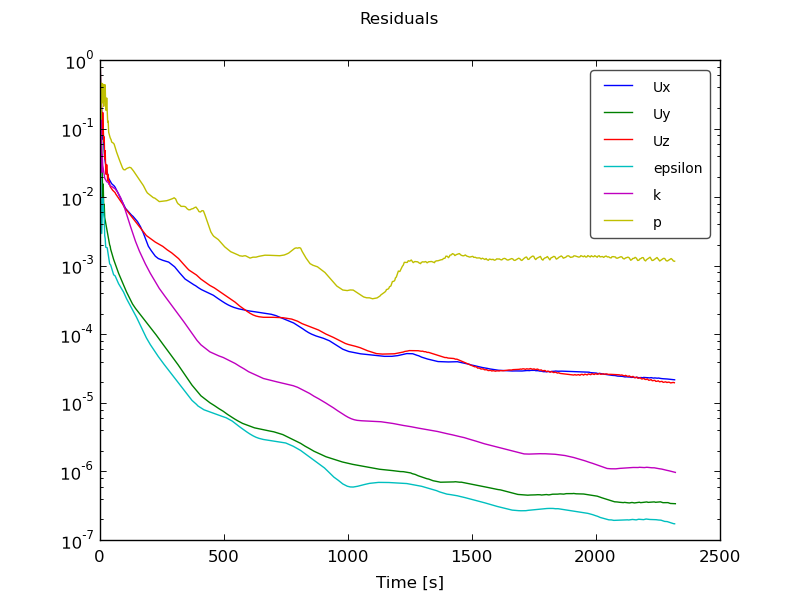
\includegraphics[width=0.48\textwidth, trim= 14mm 2mm 12mm 17mm, clip]{images/plots/validation/iterative_convergence/linear_fine}}
			\annotatedFigureBoxBlack{0.47,0.57}{0.89,0.65}{A}{0.47,0.57}%bl
	\end{annotatedFigure}}\hfil
	\centering
	\subfloat[][Volumetric flow rates obtained by the meshes above. The flow rate in the experiment was measured as \SI{0.045}{\cubic\metre\per\second}.]%
	{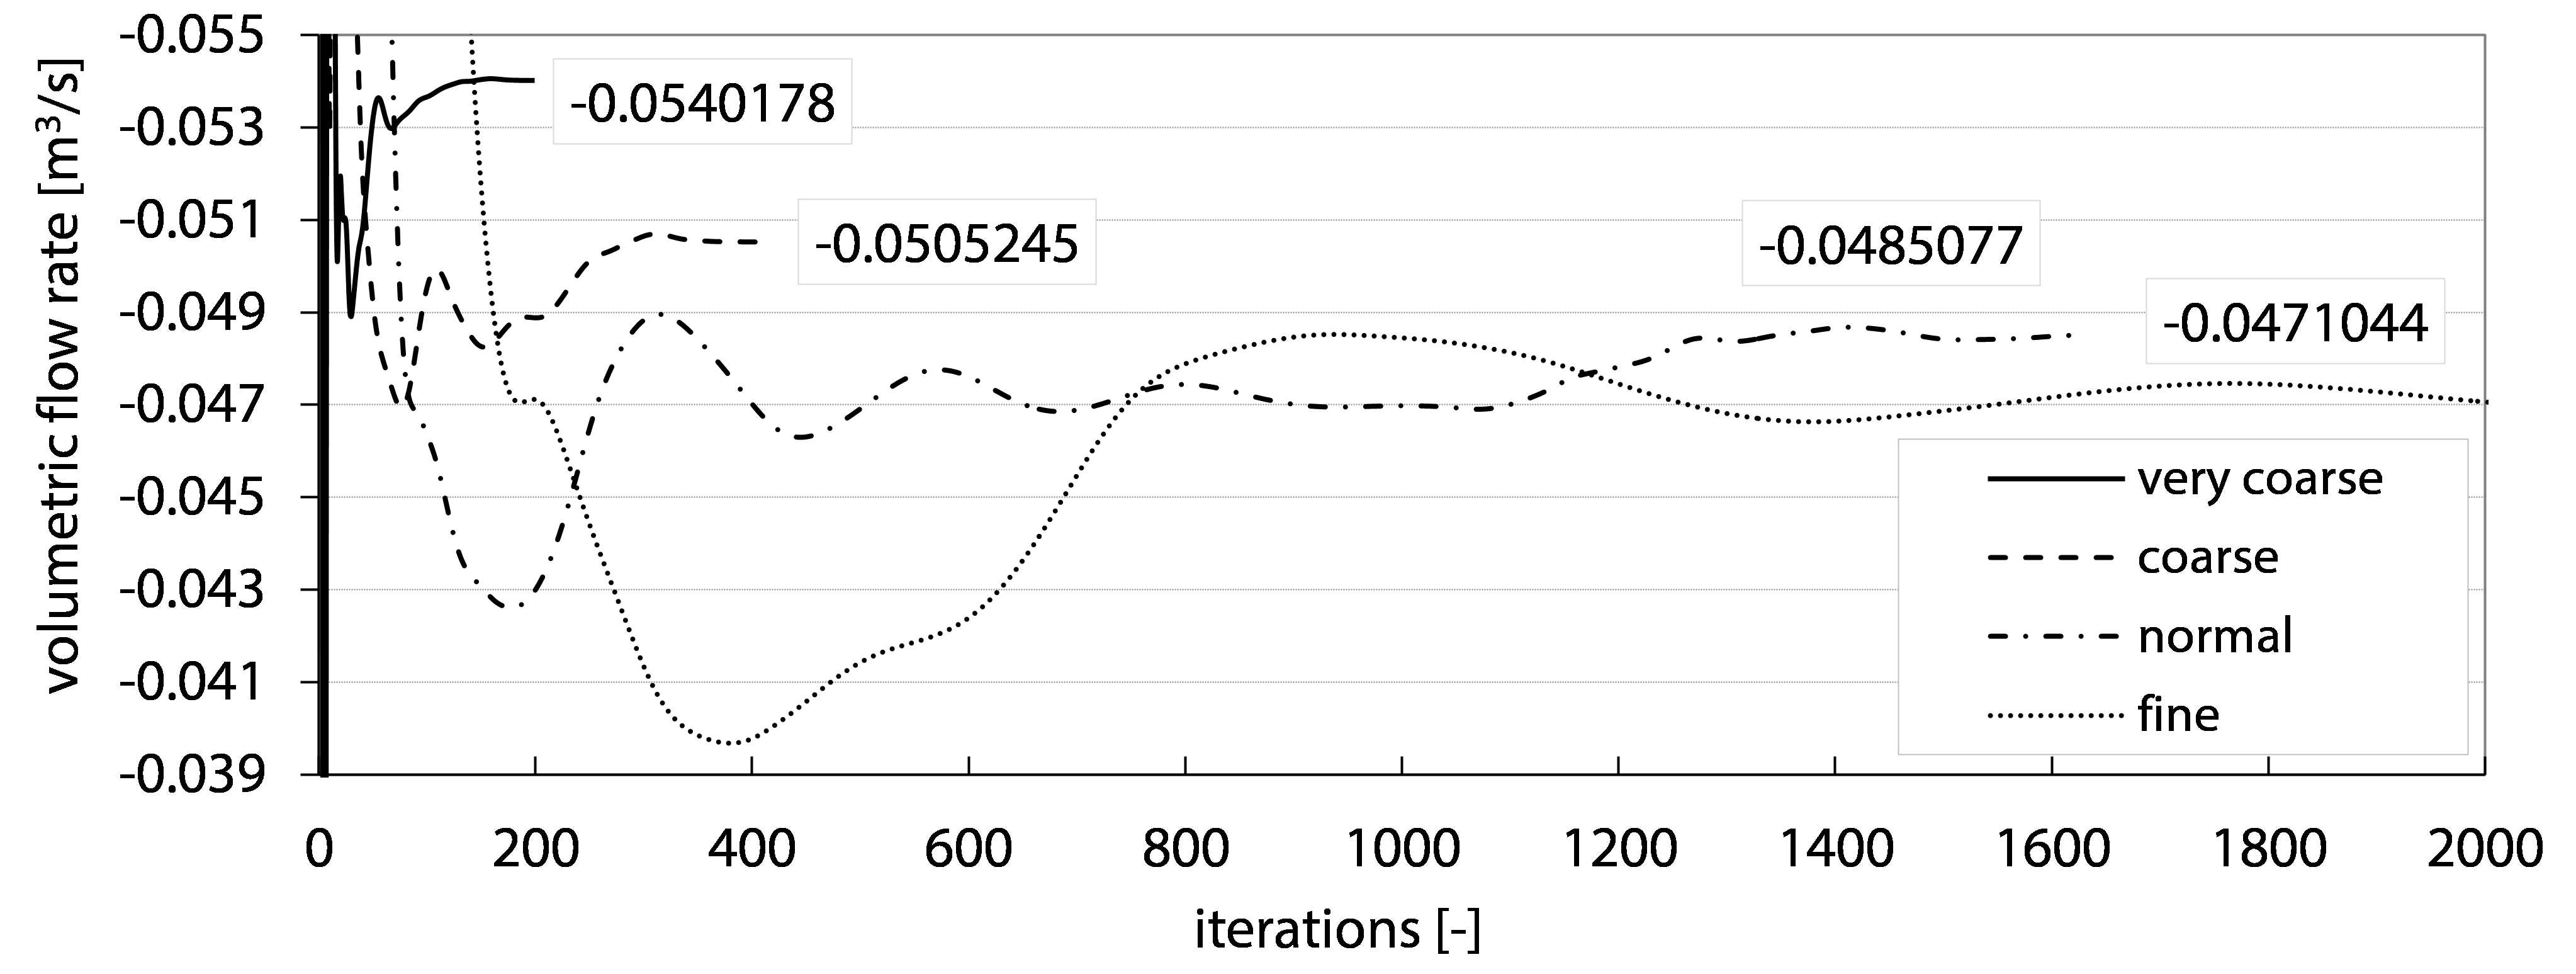
\includegraphics[width=1\linewidth, trim= 14mm 11mm 12mm 7mm, clip]{images/plots/validation/volumetric_flow_rates_grid_study}}
	\captionsetup{format=plain}%,labelsep=newline}
	\caption[Residual plots and volumetric flow rates of the mesh refinement study]{Residual plots and volumetric flow rates of the mesh refinement study. \textbf{(a-c)} The finer the mesh, the more iterations are needed to until the convergence criteria is reached. \textbf{(d)} The residuals of the \textit{fine} mesh did not reach the convergence criteria and showed oscillatory convergence for the pressure variable, see \textbf{(A)}. \textbf{(e)} Volumetric flow rates obtained by the aforementioned meshes. The convergence criteria in \fref{tab:convergence_crit_validation_study} are stringent enough to obtain stable solutions with regard to volumetric flow rates.}
	\label{fig:validation:residual_plots+volumetric_flow rates}
\end{figure}




Finally, the \textit{potentialFoam} solver should be implemented in the work-flow, which could not be done in this thesis in the interest of time.
The \textit{potentialFoam} solver provides initial fields by only solving the pressure equation of the \gls{NSE}.
Thus, it can be used as an efficient solver, initializing the velocity field for more complex solvers like \textit{simpleFoam}. 
As a result, instead of starting from a resting flow with \textit{simpleFoam}, the \textit{potentialFoam} solution may be used as an initial guess and to help to achieve convergence faster.



\FloatBarrier

%Grid study showing the discrepancies between various grids \cite{Ramponi2012}
%\clearpage
\subsubsection{Spatial convergence}
\label{sec:validation:spatial_convergence}
\index{validation!spatial convergence}

In this section, the 4 stages of mesh refinement discussed in \fref{sec:validation:mesh_fineness} are used to determine whether spatial convergence is obtained.
In doing so, one is able to determine up to which extent the mesh should be refined to ensure that  the result for a derived variable (such as the flow rate) will not change significantly with further iterations.

Along with this, another method that falls under the spatial convergence assessment method is called \gls{RE} \citep{Slater2008}. 
It predicts the variable of interest for a theoretically perfect grid with zero grid spacing\textemdash essentially a continuum\textemdash by using lower-order discrete values of that same variable.

Moreover, one is able to estimate the numerical discretization error caused by various mesh sizes. 
This allows to estimate the error due to discretization altogether. 
\Fref{tab:grid_convergence_study} shows the parameters of the 4 mesh sizes studied. 


\definecolor{light-grey}{cmyk}{0,0,0,0.10}

\begin{table}[!b]
	\small
	\centering
	\captionsetup{format=plain}
	\caption[Parameters of grid convergence study]{Parameters of grid convergence study. The study was conducted for 4 different mesh sizes: \textit{very coarse}, \textit{coarse}, \textit{normal} and \textit{fine}.  $r$ is the grid refinement ratio and $h$ is the normalized  grid spacing. Moreover, the Richardson Extrapolation (RE) predicts the flow rate for an ideal mesh (continuum), estimating the magnitude of the numerical error. $\dot{v}$ shows the flow rate through the windward opening obtained.  exp. $=$ experiment by  \citep{Jiang2003}. cont. $=$ continuum. The \textit{normal} mesh shows reasonable accuracy and is therefore chosen for further studies.}
	\label{tab:grid_convergence_study}
	\begin{tabular}{SrlrSSSSSS}
		\toprule
		{\#} & type & case                            & {cell \#} 	    & {$h$} & {$r$}  &  {$\dot{v}$ [\si{\cubic\metre\per\second}]}  & {error (exp.)} &  {error (cont.)}  &\\ \midrule
		1   &  sim.  & very coarse                 & \num{124456}     	& 8   	& 1.3 	& 0.054	& \SI{17}{\percent}  & \SI{15}{\percent} &\\%0.054017
		2   &  sim.  & coarse                        & \num{263919}     	& 4   	& 1.6 	& 0.051	& \SI{11}{\percent}  & \SI{10}{\percent}&\\%0.050524
		\rowcolor{light-grey}  3   & sim.    & normal                        & \num{1165733}   	& 2   	& 1.6 	& 0.049	&\SI{7}{\percent}   & \SI{6}{\percent}&\\%0.048507
		4   & sim.   & fine                             & \num{4940280}  	& 1   	& {-} 		& 0.047	& \SI{4}{\percent}  & \SI{3}{\percent} &\\%0.047104
		{-}  &  calc.  & RE                              & {-}       		& 0   	& {-} 		& 0.046	&  &\\%0.045752
		{-}  &  meas.  & experiment  & {-}       		& {-} 		& {-}  	& 0.045 &  &\\ \bottomrule
	\end{tabular}
\end{table}



The effective grid refinement ratio $r$ for unstructured grids is defined as:

\begin{equation}
r = \left( \frac{N_{i}}{N_{i+1}}\right)^\frac{1}{D} 
\end{equation}



